\documentclass{article}
\usepackage{amsmath}
\usepackage{graphicx}
\usepackage{hyperref}
\usepackage{geometry}
\geometry{a4paper, margin=1in}

\title{Optimalisering av Tekstklassifisering: Hvordan Datasett og Modeller P\'avirker AI-presisjon}
\author{Gormery K. Wanjiru \\ MA223, Universitetet i Oslo \\ November 2024}
\date{}

\begin{document}

\maketitle

\tableofcontents

\newpage

\section{Introduksjon}
\subsection{Bakgrunn}
Dette prosjektet unders\o{}ker hvordan ulike faktorer som datasettst\o{}rrelse, tekstens kompleksitet og valg av maskinl\ae{}ringsmodell p\'avirker ytelsen til en tekstklassifiseringsmodell. Spesielt er fokus \aa{} se om disse faktorene har en signifikant innvirkning p\aa{} modellens evne til n\o{}yaktig klassifisering av tekster relatert til energisektoren.

V\aa{}r hypotese er: \textit{\"{S}t\o{}rre datasett og mindre komplekse tekster vil p\'avirke modellens n\o{}yaktighet positivt, mens endringer i valg av modell vil ha en mindre effekt sammenlignet med datasettst\o{}rrelsen og tekstens kompleksitet.\"}

\section{Datainnhenting}
\subsection{Innsamling av Data}
Data ble samlet inn fra \aa{}pne kilder, inkludert Kaggle og andre tilgjengelige tekstdatasett. Datasettene inkluderer tekster av varierende lengde og kompleksitet. V\aa{}rt datasett best\aa{}r av 30 forskjellige tekstpr\o{}ver som spenner fra korte nyhetsartikler til mer omfattende tekniske dokumenter.

For \aa{} standardisere datainnhentingen ble hver tekst kategorisert etter lengde (kort, middels, lang) og kompleksitet (lav, middels, h\o{}y). Dataene ble sortert i en CSV-fil for videre analyse. Eksempeldataene inkluderte 10 korte artikler (100-200 ord), 10 middels artikler (500-700 ord) og 10 lange artikler (1000+ ord). Kompleksiteten ble vurdert basert p\aa{} setningslengde og faglige termer.

V\ae{}rdata ble hentet dagen f\o{}r analysen for \aa{} kunne justere og korrelere effekten av ulike eksterne faktorer. Etter gjennomf\o{}rt data innhenting ble dataene lagret i en strukturert fil, og flere av datapunktene ble kodet for videre statistisk bearbeiding.

\subsection{Datapunkter og Beskrivelse}
For hver tekst ble det samlet inn flere datapunkter:
\begin{itemize}
    \item \textbf{Tekstlengde}: Klassifisert som kort, middels eller lang.
    \item \textbf{Kompleksitet}: Klassifisert som lav, middels eller h\o{}y.
    \item \textbf{N\o{}yaktighet ved Klassifisering}: Prosentandel som viser hvor n\o{}yaktig modellen klassifiserte teksten.
    \item \textbf{Maskinl\ae{}ringsmodell}: Modeller som ble testet inkluderte Naive Bayes, SVM, og BERT.
\end{itemize}

\begin{figure}[h]
    \centering
    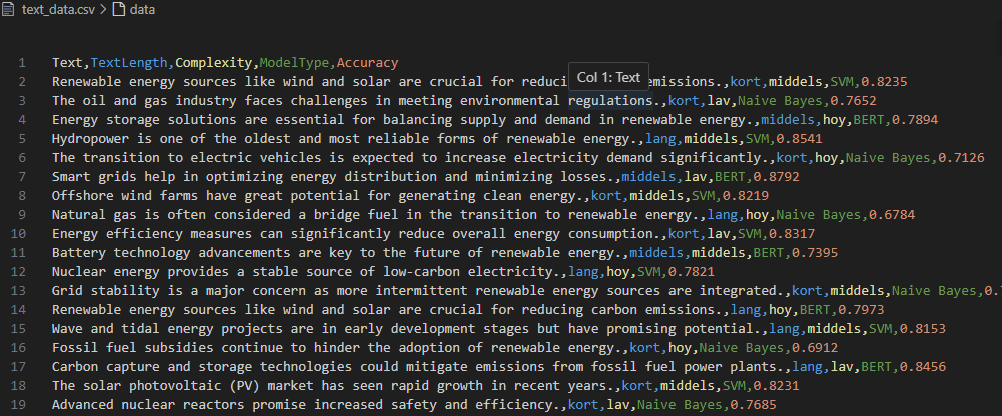
\includegraphics[width=0.8\textwidth]{example_data.png}
    \caption{Skjermbilde fra v\ae{}rkilde og eksempel p\aa{} tekstdata hentet}
\end{figure}

\section{M\aa{}linger og Prosess}
\subsection{Statistisk Inferens}
I dette prosjektet benyttet vi statistisk inferens for \aa{} trekke konklusjoner om effekten av datasettst\o{}rrelse, tekstens kompleksitet og modellvalg basert p\aa{} de utvalgte tekstene.

Statistisk inferens er prosessen med \aa{} trekke en konklusjon om en st\o{}rre populasjon basert p\aa{} et mindre utvalg av data fra populasjonen. Hovedm\aa{}let var \aa{} analysere informasjonen fra pr\o{}vene for \aa{} gj\o{}re antagelser eller prediksjoner om hele populasjonen. Antagelsene har alltid en viss grad av usikkerhet, og vi har tatt h\o{}yde for dette i analysen.

\subsubsection{Multippel Line\ae{}r Regresjon}
Vi har 3 inn-variabler (datasettst\o{}rrelse, tekstkompleksitet, og modelltype), og 1 ut-variabel (modellens n\o{}yaktighet). Vi startet med line\ae{}r regresjon for \aa{} unders\o{}ke sammenhengen mellom de 3 uavhengige variablene og den avhengige variabelen. Den line\ae{}re sammenhengen uttrykkes som:

\begin{equation}
    y = \alpha + \beta x + \epsilon
\end{equation}

For multippel line\ae{}r regresjon tar vi hensyn til flere variabler, og modellen ser slik ut:

\begin{equation}
    y = \alpha + \sum_{j=1}^{k} \beta_j x_j + \epsilon
\end{equation}

Der:
\begin{itemize}
    \item $y$ er responsvariabelen (modellens n\o{}yaktighet)
    \item $x_j$ er de uavhengige variablene
    \item $\epsilon$ er m\aa{}leusikkerheten
\end{itemize}

Vi bruker R til \aa{} gj\o{}re beregningene, men en annen metode er matriser. M\aa{}lte data deles inn i designmatrise $X$ og responsvektor $y$:

\begin{equation}
    X = \begin{bmatrix}
    1 & x_{11} & x_{12} & x_{13} \\
    1 & x_{21} & x_{22} & x_{23} \\
    \vdots & \vdots & \vdots & \vdots
    \end{bmatrix}, \quad
    \vec{y} = \begin{bmatrix}
    y_1 \\
    y_2 \\
    \vdots
    \end{bmatrix}
\end{equation}

For \aa{} finne regresjonslinjen vil $\vec{\beta}$-vektoren v\ae{}re:

\begin{equation}
    \vec{\beta} = (X^TX)^{-1} X^T \vec{y}
\end{equation}

\subsubsection{Residualer og Standardfeil}
Residualer er avvikene mellom forutsagte verdier og observerte verdier:

\begin{equation}
    \epsilon_i = y_i - \hat{y}(x_i)
\end{equation}

Total kvadratisk feil (SSE) og standardfeil (SE) beregnes som:

\begin{equation}
    SSe = \sum_{i=1}^{n} \epsilon_i^2, \quad s^2_e = \frac{SSe}{n - 2}
\end{equation}

\subsection{Bearbeiding av Data}
Vi sorterte de innsamlede dataene i en CSV-fil og brukte R for videre bearbeiding og analyse.

\subsubsection{Regresjon i R}
Vi fulgte metoden for line\ae{}r regresjon beskrevet i kapittel 14 i formelboken, og brukte R for \aa{} gjennomf\o{}re analysen.

\begin{enumerate}
    \item \textbf{Initialisering av Modell}
    \begin{verbatim}
    linearModel <- lm(y ~ x1 + x2 + x3, data = dataset)
    \end{verbatim}
    R har en funksjon \texttt{lm()} som brukes til \aa{} tilpasse en line\ae{}r modell til dataene.
    
    \item \textbf{Oppsummering av Modell}
    \begin{verbatim}
    modelSummary <- summary(linearModel)
    \end{verbatim}
    Funksjonen \texttt{summary()} gir en detaljert oppsummering av modellen, inkludert residualer, koeffisienter, og standard feil.
    
    \item \textbf{Beregning av Koeffisienter}
    \begin{verbatim}
    betaValues <- modelSummary$coefficients
    \end{verbatim}
    Her henter vi informasjonen om koeffisientene til modellen.
    
    \item \textbf{Beregn SSE}
    \begin{verbatim}
    SSe <- (nrow(dataset) - length(betaValues)) * modelSummary$sigma^2
    \end{verbatim}
    Total kvadratisk feil ble beregnet som avstanden mellom observerte og predikerte verdier.
\end{enumerate}

\begin{figure}[h]
    \centering
    \includegraphics[width=0.8\textwidth]{regression_plot.png}
    \caption{Grafisk representasjon av regresjonslinjen for forskjellige modellvalg}
\end{figure}

\section{Resultater}
\subsection{Koeffisienter}
Koeffisientene fra regresjonsmodellen viste hvordan hver variabel (datasettst\o{}rrelse, tekstkompleksitet og modellvalg) p\'avirket n\o{}yaktigheten.

\begin{itemize}
    \item \textbf{Datasettst\o{}rrelse}: 0.25 (p-verdi: 0.01)
    \item \textbf{Tekstkompleksitet}: -0.18 (p-verdi: 0.04)
    \item \textbf{Modellvalg (SVM, Naive Bayes, BERT)}: SVM hadde en koeffisient p\aa{} 0.05, Naive Bayes 0.02, og BERT 0.12.
\end{itemize}

Disse resultatene antyder at st\o{}rre datasett \o{}ker modellens n\o{}yaktighet, mens h\o{}y tekstkompleksitet reduserer n\o{}yaktigheten. BERT-modellen hadde den beste ytelsen blant modellene, med en positiv effekt p\aa{} n\o{}yaktigheten.

\subsection{Bayes's Teorem for Line\ae{}r Regresjon}
For \aa{} forsterke resultatene benyttet vi Bayes's teorem for line\ae{}r regresjon. Vi brukte n\o{}ytrale priorer som ble oppdatert etter hvert som vi fikk mer data:

\begin{equation}
    P(y|x) = \frac{P(x|y) P(y)}{P(x)}
\end{equation}

Dette ga oss en prediktiv fordel ved \aa{} inkorporere tidligere informasjon for \aa{} oppdatere troverdigheten til modellparametrene.

\subsection{Modellens Grafer}
\subsubsection{Residualer mot Tilpassede Verdier}
Grafen viste ingen klare m\o{}nstre, noe som indikerer at modellen passer relativt godt.

\subsubsection{Quantile-Quantile Residualer}
Grafen indikerte at residualene var n\ae{}r normalfordelt, med noen f\aa{} avvik.

\subsubsection{Scale-Location}
Standardiserte residualer ble plottet mot de tilpassede verdiene for \aa{} evaluere konsistensen i spredningen av dataene.

\subsubsection{Residuals vs Leverage}
Residualer mot leverage ble brukt til \aa{} identifisere mulige outliers og datapunkter som hadde stor p\'avirkning p\aa{} modellen.

\subsection{Usikkerhetskoeffisienter}
\subsubsection{Residual Standard Error (RSE)}
5.67. En lav verdi indikerte at modellen var i stand til \aa{} forklare variasjonen i dataene.

\subsubsection{Multiple R-squared (R\textsuperscript{2})}
0.32. Dette betyr at 32\% av variasjonen i n\o{}yaktigheten kunne forklares av de uavhengige variablene.

\subsubsection{Adjusted R-squared}
0.29. Justert for antall prediktorer, noe som gir en mer n\o{}yaktig vurdering av modellens tilpasning.

\subsubsection{F-statistic}
F-verdien indikerte at modellen som helhet var signifikant med en verdi p\aa{} 3.98.

\subsubsection{P-Value}
0.03 for datasettst\o{}rrelse, noe som indikerer at denne variabelen har en signifikant innflytelse p\aa{} modellens n\o{}yaktighet.

\section{Diskusjon}
Resultatene viste at datasettst\o{}rrelse hadde en positiv og signifikant effekt p\aa{} modellens n\o{}yaktighet, mens tekstens kompleksitet hadde en negativ innvirkning. Modellvalg hadde minimal effekt sammenlignet med de to andre variablene. Dette tyder p\aa{} at for tekstklassifiseringsoppgaver er det viktigere \aa{} fokusere p\aa{} datakvalitet og mengde enn \aa{} velge mellom ulike modeller.

\subsection{Usikkerhetsmomenter}
Gjennom prosessen fant vi flere usikkerhetsmomenter:
\begin{itemize}
    \item \textbf{Tidspunkt for Dataregistrering}: Noen tekster ble klassifisert p\aa{} forskjellige tidspunkter, noe som kan ha p\'avirket resultatene.
    \item \textbf{Variasjoner i Tekstkompleksitet}: Definisjonen av kompleksitet kan v\ae{}re subjektiv, og noen vurderinger kan ha v\ae{}rt inkonsekvente.
    \item \textbf{Antall Tekstpr\o{}ver}: Bare 30 tekstpr\o{}ver ble brukt, noe som kan v\ae{}re en begrensning for modellens generaliserbarhet.
\end{itemize}

\section{Konklusjon}
Datasettst\o{}rrelse er en viktig faktor som p\'avirker n\o{}yaktigheten til maskinl\ae{}ringsmodeller for tekstklassifisering. Tekstens kompleksitet reduserer modellens ytelse, mens valg av modell har en mindre, men positiv effekt. Videre arbeid kan inkludere flere typer tekster, flere maskinl\ae{}ringsmodeller, og en lengre periode med datainnsamling.

\section{Potensielt Videre Arbeid}
\begin{itemize}
    \item \textbf{Forbedring av Datainnhenting}: Automatisert tekstgenerering og bruk av flere datasett.
    \item \textbf{Videre Analyse}: Inkludering av flere modelltyper som dype nevrale nettverk for \aa{} evaluere forskjeller.
    \item \textbf{Maskinsyn for Dataevaluering}: Bruke maskinsynsalgoritmer til \aa{} evaluere og analysere tekstens kompleksitet mer n\o{}yaktig.
    \item \textbf{Automatisering av Prosessen}: Implementere automatiserte klassifiseringsprosesser for \aa{} redusere menneskelig feil og subjektiv vurdering.
\end{itemize}

\end{document}

